%
% Gradient Info
\tikzset {_2wjvdlgsv/.code = {\pgfsetadditionalshadetransform{ \pgftransformshift{\pgfpoint{0 bp } { 0 bp }  }  \pgftransformrotate{-45 }  \pgftransformscale{2 }  }}}
\pgfdeclarehorizontalshading{_189nw8o3l}{150bp}{rgb(0bp)=(0.03,0.22,0.4);
rgb(37.5bp)=(0.03,0.22,0.4);
rgb(43.86904580252511bp)=(0.03,0.22,0.4);
rgb(62.5bp)=(0.05,0.36,0.63);
rgb(100bp)=(0.05,0.36,0.63)}
\tikzset{every picture/.style={line width=0.75pt}} %set default line width to 0.75pt         
%
%
\begin{equation}
\label{eq:demo-tikz-eq}
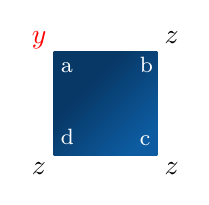
\begin{tikzpicture}[baseline={([yshift=-.5ex]current bounding box.center)},x=0.75pt,y=0.75pt,yscale=-1,xscale=1]

%Shape: Square [id:dp9442510713449753] 
\draw  [draw opacity=0][shading=_189nw8o3l,_2wjvdlgsv] (20,20) -- (70,20) -- (70,70) -- (20,70) -- cycle ;

% Text Node
\draw (8,9) node [anchor=north west][inner sep=0.75pt]    {$\textcolor{red}{y}$};
% Text Node
\draw (72,9) node [anchor=north west][inner sep=0.75pt]    {$z$};
% Text Node
\draw (8,72) node [anchor=north west][inner sep=0.75pt]    {$z$};
% Text Node
\draw (72,72) node [anchor=north west][inner sep=0.75pt]    {$z$};
% Text Node
\draw (22,24) node [anchor=north west][inner sep=0.75pt]  [font=\footnotesize,color={rgb, 255:red, 255; green, 255; blue, 255 }  ,opacity=1 ] [align=left] {a};
% Text Node
\draw (60,21) node [anchor=north west][inner sep=0.75pt]  [font=\footnotesize,color={rgb, 255:red, 255; green, 255; blue, 255 }  ,opacity=1 ] [align=left] {b};
% Text Node
\draw (60,59) node [anchor=north west][inner sep=0.75pt]  [font=\footnotesize,color={rgb, 255:red, 255; green, 255; blue, 255 }  ,opacity=1 ] [align=left] {c};
% Text Node
\draw (22,56) node [anchor=north west][inner sep=0.75pt]  [font=\footnotesize,color={rgb, 255:red, 255; green, 255; blue, 255 }  ,opacity=1 ] [align=left] {d};

\end{tikzpicture}
\equiv \textcolor{red}{\hat\sigma_y^{(a)}}\otimes\hat\sigma_z^{(b)}\otimes\hat\sigma_z^{(c)}\otimes\hat\sigma_z^{(d)}
\end{equation}